%% ============================================================
% f2012_sichuan_sci_q04_square.tex
%% 2012 四川卷（理科）第 4 题 正方形 ABCD，延长 BA 至 E 使 AE=1
%% 来源 PDF：普通高考/2012/2012四川理.pdf 第 1 页（印面 771）第 1 栏
%% 坐标取自原页矢量层（bp），原点为图区左上角 (170.0,355.0)，y 向下。
%% ============================================================
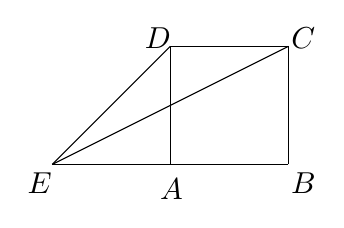
\begin{tikzpicture}[x=1bp,y=-1bp,
  every node/.style={inner sep=0,font=\fontsize{10.5pt}{12.6pt}\selectfont},
  line cap=butt, line join=miter]
  \draw[line width=0.398bp] (10.828,53.777) -- (95.836,53.777);
  \draw[line width=0.398bp] (95.836,11.273) -- (53.332,11.273);
  \draw[line width=0.398bp] (10.828,53.777) -- (95.836,11.273);
  \draw[line width=0.398bp] (95.836,53.777) -- (95.836,11.273);
  \draw[line width=0.398bp] (10.828,53.777) -- (53.332,11.273);
  \draw[line width=0.398bp] (53.332,53.777) -- (53.332,11.273);
  \node[anchor=base west] at (43.99,12.0) {$D$};
  \node[anchor=base west] at (96.74,12.0) {$C$};
  \node[anchor=base west] at (1.79,64.38) {$E$};
  \node[anchor=base west] at (49.48,66.43) {$A$};
  \node[anchor=base west] at (96.62,64.38) {$B$};
\end{tikzpicture}
